\section{Advective-Reactive \texorpdfstring{$r$}{r}-process}\label{sec:ar_rprocess}

Advective-reactive nucleosynthesis refers to the generic case where any mixing interaction timescale is similar to the reaction timescale.
Here I present preliminary work done with Dr. Herwig analyzing a new scenario beyond the post-processed O-shell.

\begin{itemize}
    \item do I have to mention that this work was done with Falk more directly
    \item Rodrigo black hole paper?
    \item Work was done to estimate both the mixing and nuclear timescale
    \item Basically found the fraction of trajectories where exchanging mass occurs on the a-r timescale.
    \item How many freaking r-process papers do I really need to cite here
\end{itemize}

\begin{figure}
\label{fig:in_timescale}
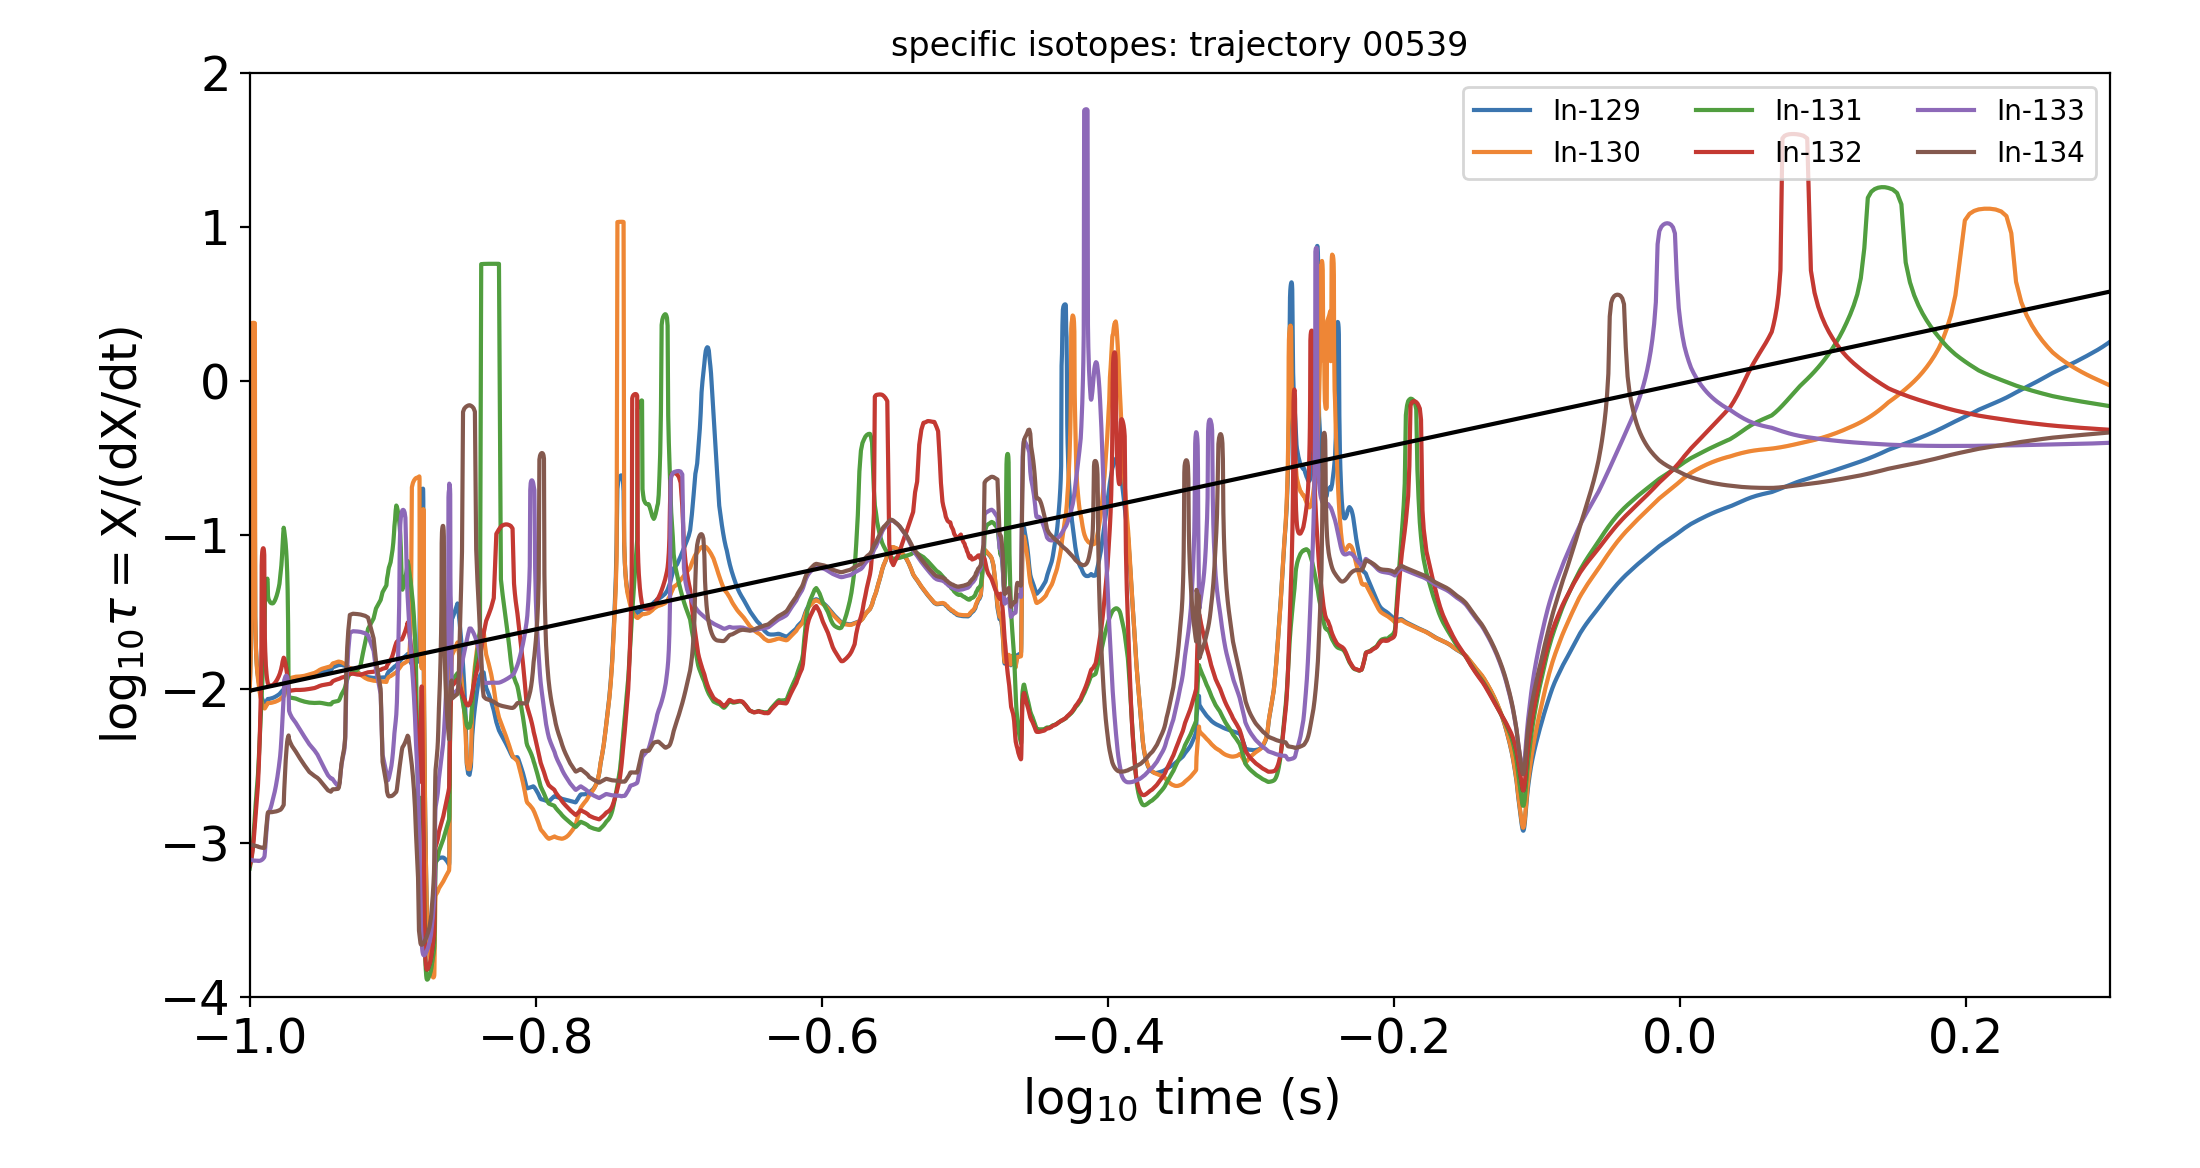
\includegraphics[width=\textwidth]{chapters/3/figures/in_timescale.png}
\caption{In isotope timescale.}
\end{figure}

\begin{figure}
\label{fig:pairwise}
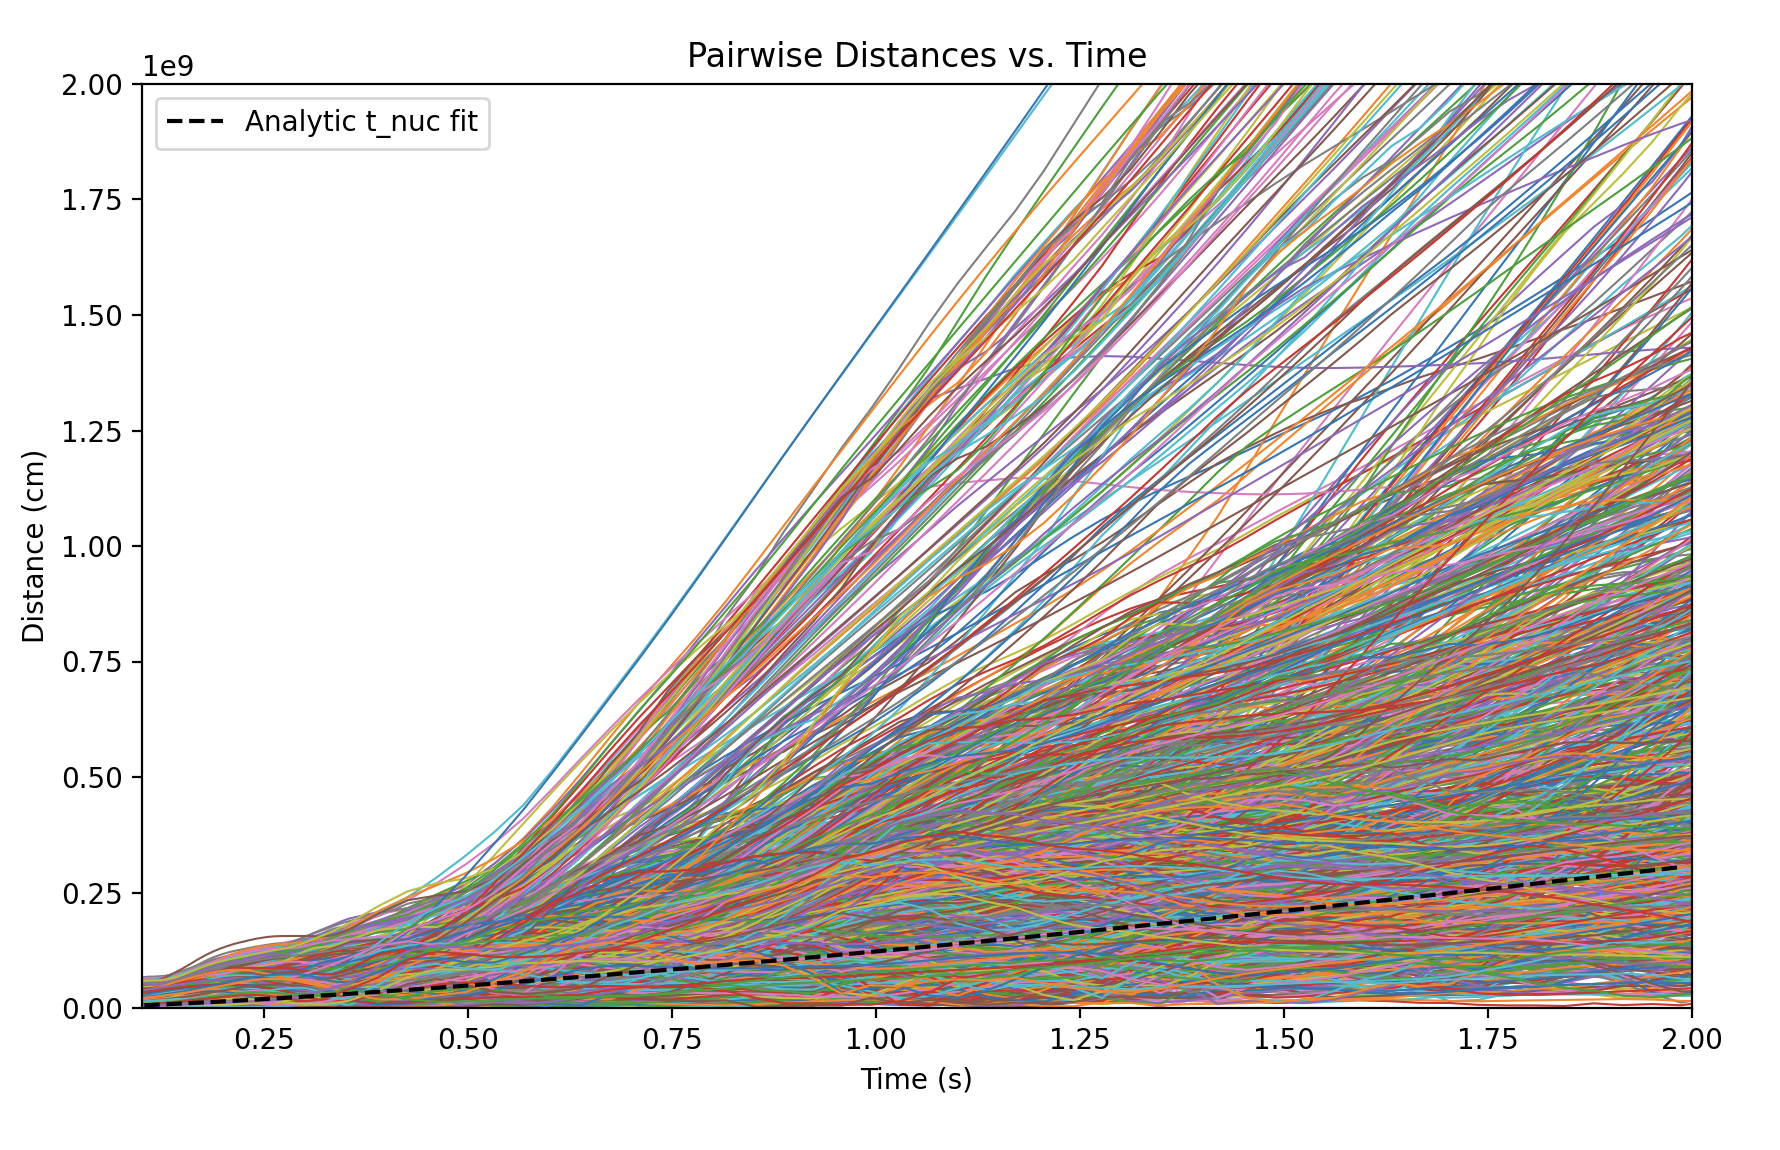
\includegraphics[width=\textwidth]{chapters/3/figures/pairwise.png}
\caption{Pairwise distance.}
\end{figure}

\begin{figure}
\label{fig:frac_exchanging}
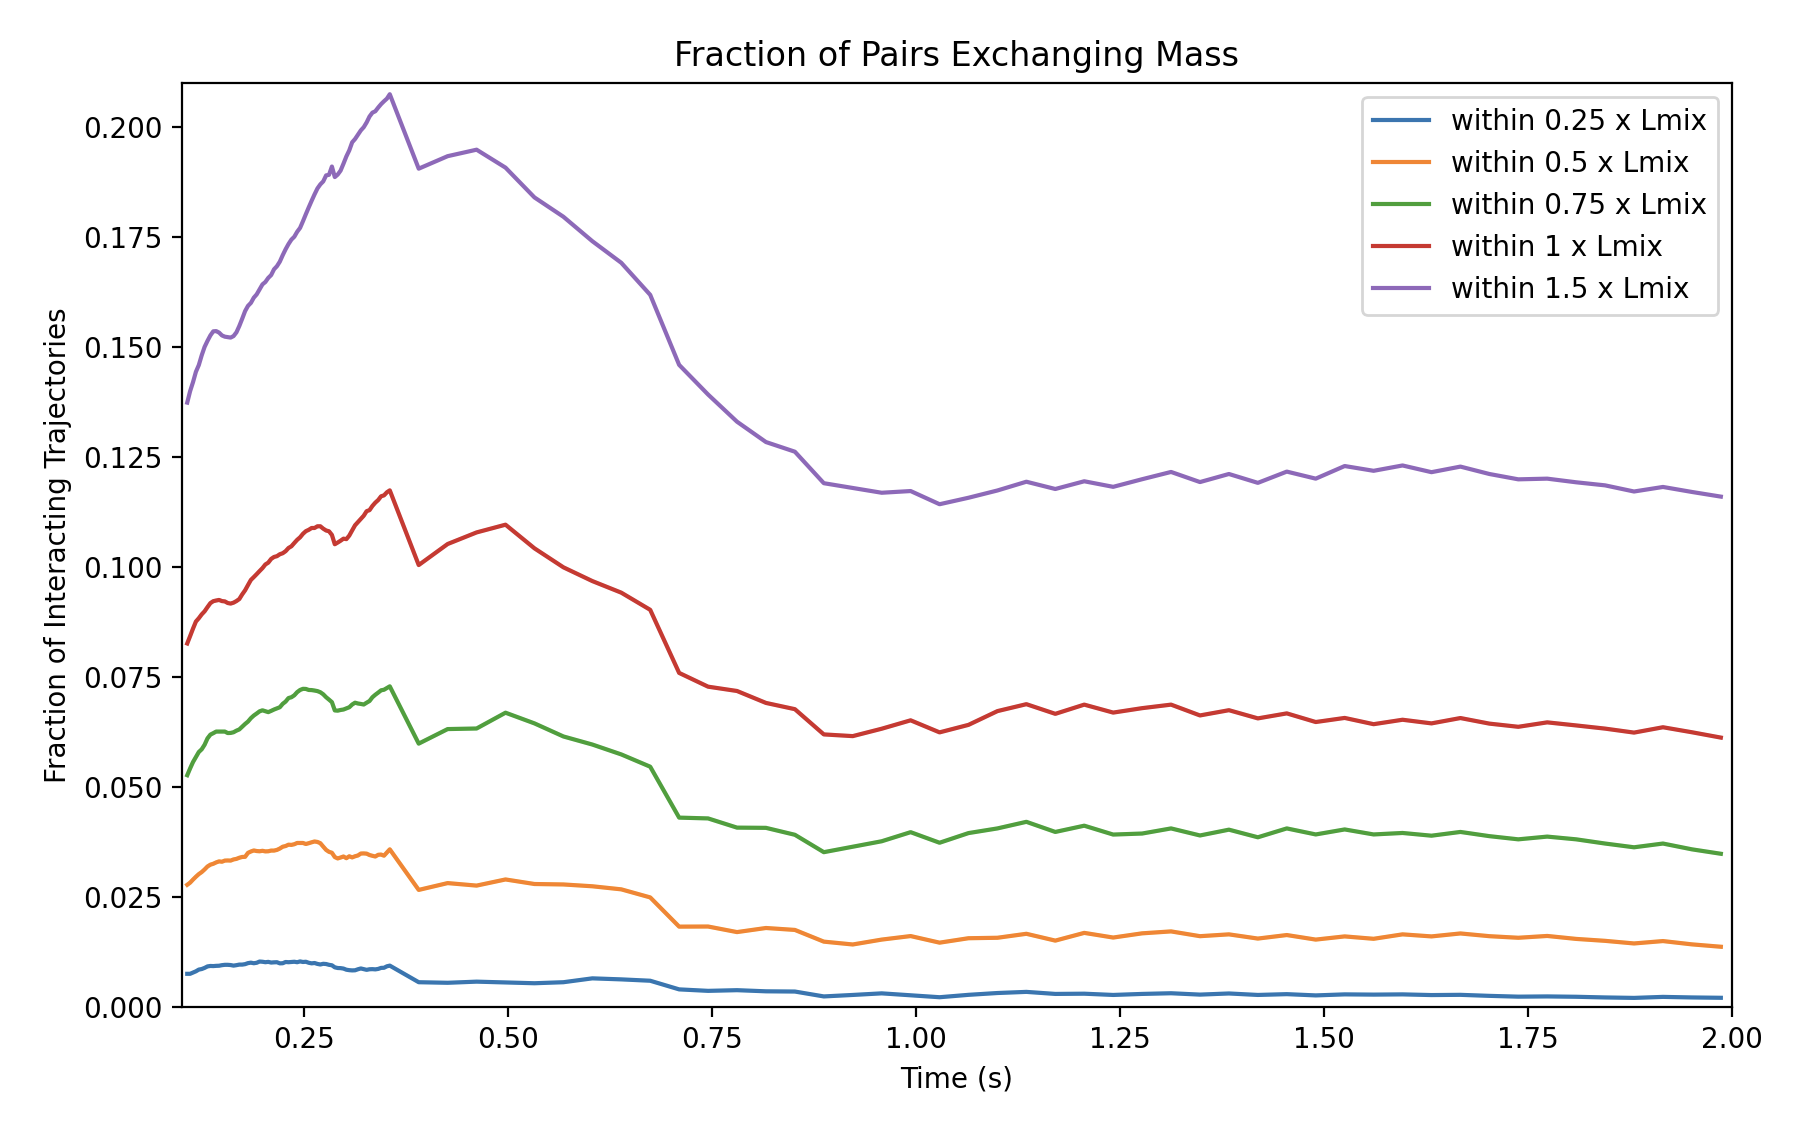
\includegraphics[width=\textwidth]{chapters/3/figures/frac_exchanging.png}
\caption{Fraction of exchanging mass.}
\end{figure}